\documentclass[11pt]{article}
\input{/Users/markwang/.preamble}
\begin{document}



\begin{enumerate}
    \item As above, assume we have 250 words in the dictionary and use the previous 3 words as inputs. Suppose we use a 16-dimensional word embedding and a hidden layer with 128 units. The trainable parameters of the model consist of 3 weight matrices and 2 sets of biases. What is the total number of trainable parameters in the model? Which part of the model has the largest number of trainable parameters?
    \begin{solution}
        Then dimension of weight matrices and biases are 
        \[
            \underset{250\times 16}{word\_embedding\_weights}
            \quad \quad 
            \underset{128\times 48}{embed\_to\_hid\_weights}
            \quad \quad 
            \underset{128\times 1}{hid\_bias}
        \]
        \[
            \underset{250\times 128}{hid\_to\_outputs\_weights}
            \quad \quad 
            \underset{250\times 1}{output\_bias}    
        \]
        Total number of trainable parameter is 
        \[
            250\times 16 + 128 \times 48 + 128 \times 1 + 250 \times 128 + 250 \times 1 = 42522
        \]
        The model has largest number of trainable parameters in matrix \textbf{hid\_to\_outputs\_weights}
    \end{solution}
    \item Another method for predicting the next word is an n-gram model, which was mentioned in Lecture 7. If we wanted to use an n-gram model with the same context length as our network, we’d need to store the counts of all possible 4-grams. If we stored all the counts explicitly, how many entries would this table have? \\ 
    Context length is 3. The size of conditional probability table of a 4-grams model is given by
    \[
        250  \times 250 \times 250 \times 250 = 3906250000
    \]
    \item A printout of your code for the two methods you had to implement: \texttt{Model.compute\_loss\_derivative} and \texttt{Model.back\_propagate}. Please do not include any other code. 
    \begin{center}
        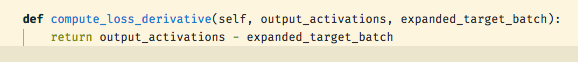
\includegraphics[width=15cm]{codeblock1.png}
        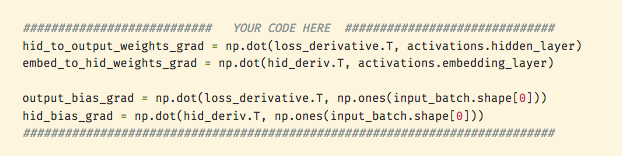
\includegraphics[width=15cm]{codeblock2.png}
    \end{center}
    \item The output of the function \texttt{checking.print\_gradients}.
    \begin{center}
        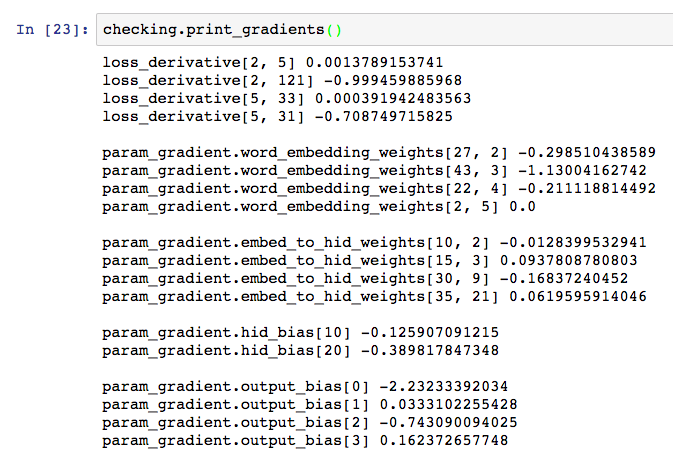
\includegraphics[width=15cm]{print_gradient.png}
    \end{center}
    \item Pick three words from the vocabulary that go well together. Use the model to predict the next word. Does the model give sensible predictions?  \\ 
    The model does give sensible predictions. Especially with $\texttt{city of new}$, $\texttt{york}$ is the most probable output with $p=0.99$. Even without appearing in the training dataset, $\texttt{government of united}$ admits a reasonable prediction where $\texttt{states}$ is third most probable prediction, however with low confidence.
    \item Plot the 2-dimensional visualization using the method $\texttt{Model.tsne\_plot}$. Look at the plot and find a few clusters of related words. What do the words in each cluster have in common? \\ 
    As an example, $\texttt{what, who, where, when, how}$ and $\texttt{can, do, does, will, should}$ form their respective clusters. It seems that each cluster consists of words that function in similar ways grammatically. More specifically, words in a cluster can oftern be substituted with other words in the same cluster without rendering the sentence from being grammatically incorrect.
    \item Are the words \texttt{new} and \texttt{york} close together in the learned representation? Why or why not? \\
    $\texttt{model.word\_distance("new", "york")}$ outputs 4.14. Calling $\texttt{display\_nearest\_words}$ on both \texttt{new} and \texttt{york} showed that they are not $k=10$ nearest words of each other. They are not close together in the learned representation. They dont seem to be close together in tsne plot. It's reasonable since they serve different grammatical function, one being an adjetive and the other a noun. 
    \item Which pair of words is closer together in the learned representation: (\texttt{government, political}), or (\texttt{government, university})? Why do you think this is? \\ 
    (\texttt{government, university}) because they are often substitutable while maintaining grammatical correctness, both are noun and functions similarly in a sentence.
\end{enumerate}



 


\end{document}
